\chapter{VarBench: variational benchmarks for quantum many-body systems}
\label{ch:varbench}

The previous chapters have introduced multiple variational methods for quantum many-body systems, including variational Monte Carlo (VMC) in \cref{ch:vmc} and tensor networks (TNs) in \cref{ch:tn}, each with its own appropriate use cases, as well as trade off between accuracy and computational cost. When different methods are applied to the same physical system, there is a simple criterion to assess their performances: A lower variational energy indicates that the method approximates the true ground state more accurately. Besides that, it is also attempting to compare the performances of one method on different physical systems, or compare the universal applicability of two methods on multiple systems. Therefore, we require a metric that can be compared both between methods and between systems.

In the following, we present the metric proposed in Ref.~\cite{wu2023variational}, namely V-score, which is used in an extensive project to benchmark the performances of variational methods on a diverse variety of physical systems. Moreover, it can measure the hardness of simulating a physical system, which identifies certain hard systems that are not yet solved by available computational techniques.

\section{V-score: universal metric for variational accuracy}

It has been widely observed that when a variational state is sufficiently close to the ground state, the variance of the variational energy $\Var E = \ev{\hat{H}^2} - \ev{\hat{H}}^2$ scales linearly with the difference between the variational energy $E$ and the ground state energy $E_0$~\cite{kwon1993, imada2000, sorella2001}:
\begin{equation}
E  - E_0 = A \Var E + O\left( (\Var E)^2 \right),
\label{eq:var-linear}
\end{equation}
where $A$ is a coefficient depending on the properties of the Hamiltonian $\hat{H}$ and the variational state $\ket{psi}$. For example, in a simple two-state system as discussed in \cref{eq:var-two-states}, we have
\begin{equation}
A = \frac{1}{E_1 - E_0}.
\end{equation}
For general systems with more energy levels, Ref.~\cite{taddei2015iterative} has given more rigorous conditions of ``sufficiently close'' to hold \cref{eq:var-linear}, which are usually satisfied in computational studies. It has been a common practice to linearly extrapolate $E$ as a function of $\Var E$, and obtain an estimation of $E_0$ at $\Var E = 0$. Therefore, even though we do not know the true ground state $E_0$, the variance can indicate the accuracy of approximating the given Hamiltonian, and we seek for a metric proportional to it.

The metric should be a dimensionless number, so we normalize the variance by the variational energy and obtain $\frac{\Var E}{E^2}$. Moreover, it should not scale with the system size $N$. The energy $E$ scales linearly with $N$, as it is an extensive quantity for all physical systems of our interest. The variance $\Var E$ also scales linearly with $N$ if the Hamiltonian satisfies the following clustering property~\cite{park1995uniqueness, nachtergaele2006lieb, hastings2006spectral}: The Hamiltonian can be written as a sum of $N$ terms labeled by the site index $i$,
\begin{equation}
\hat{H} = \sum_{i = 1}^N \hat{h}_i,
\end{equation}
and the correlations between these terms decay quickly enough with the spatial distance of the sites,
\begin{equation}
\left| \ev*{\hat{h}_i \hat{h}_j} - \ev*{\hat{h}_i}\!\ev*{\hat{h}_j} \right| \le \frac{A_\text{corr}}{d^{D + \epsilon}(i, j)},
\end{equation}
where $A_\text{corr}$ is a constant for all $i, j$, $d(i, j)$ is the distance between the sites $i, j$, $D$ is the spatial dimension, and $\epsilon$ is a small positive number for all $i, j$. All physical systems of our interest has this clustering property, and we note that for non-critical systems the correlations decay exponentially with the distance. Therefore, we scale the variance by $N$ and obtain $\frac{N\,\Var E}{E^2}$, which is asymptotically independent of $N$.

A remaining issue is that we can arbitrarily shift the Hamiltonian by a constant: $\hat{H} \gets \hat{H} + C$, which does not change any physical property of the system, and our metric should be invariant under this shift. Therefore, we define a zero point of energy $E_\infty$, and replace $E$ by $E - E_\infty$. For spin and fermionic systems with a finite number of energy levels per site, $E_\infty$ is defined to be the expected energy of a random state in the Hilbert space, and we are sure that a variational state after optimization typically has a lower energy than a random state. It is equivalent to the expected energy of a thermal state at infinite temperature, which can be derived from the trace of the Hamiltonian:
\begin{equation}
E_\infty = \frac{\Tr \hat{H}}{\dim \calH},
\label{eq:E-infty-trace}
\end{equation}
where $\dim \calH$ is the dimension of the Hilbert, or the Hilbert subspace for fermionic systems when the number of fermions is fixed. It can be analytically derived for simple Hamiltonians, or numerically evaluated using Monte Carlo sampling. However, it remains an open question to define $E_\infty$ for bosonic systems, because there are infinitely many energy levels per site. We may define it with a cutoff of physically relevant energy levels, or a mean-field energy, but there is not yet an intuitive definition that is consistent with spin and fermionic systems.

The resulting definition of the metric for variational accuracy, namely V-score, is
\begin{equation}
\text{V-score} = \frac{N\,\Var E}{(E - E_\infty)^2}.
\label{eq:v-score}
\end{equation}
It is dimensionless, asymptotically independent of the system size, and invariant to the energy shift. Moreover, it can be efficiently evaluated without knowing the ground state energy. Substituting \cref{eq:var-linear,eq:v-score} into the energy relative error $\frac{E - E_0}{|E_0 - E_\infty|}$, we can obtain the linear relation
\begin{align}
\frac{E - E_0}{|E_0 - E_\infty|} &= B\,\text{V-score} + O(\text{V-score}^2), \label{eq:v-score-rel-err} \\
B &= \frac{A (E - E_\infty)^2}{N |E_0 - E_\infty|},
\end{align}
where $A$ has the dimension of $E^{-1}$ and is asymptotically independent of $N$. For any Hamiltonian with the clustering property and any variational state converging to the ground state, the magnitude of $B$ will not be too far from $1$. Therefore, the V-score can be a universal metric to predict the energy relative error in variational approximation.

It is worth discussing the possibilities for the V-score to underestimate or overestimate the energy relative error. An intuitive case of the underestimation is when the variational state converges to an excited state, as $\Var E$ under any excited state is zero. This situation can be detected by applying the symmetries of the ground state, or repeating the optimization with different initial parameters. Another case is the mode collapse discussed in \cref{sec:vmc-var}, where we estimate $\Var E$ using $|E_\text{loc}(\vs)|^2$, and it can be detected by actually evaluating the matrix elements of $\hat{H}^2$.

For the extent that the V-score can overestimate the energy relative error, it is proven that
\begin{equation}
\frac{\text{V-score}}{(E - E_0) / (E_\infty - E_0)} \le N \frac{(E_\infty - E_0) (E_\text{M} - E)}{(E_\infty - E)^2},
\label{eq:v-score-bound}
\end{equation}
where $E_\text{M}$ is the highest energy level of the system, and the variational state can be an arbitrary linear combination of the eigenstates. This upper bound is not very ideal as it is linear in $N$, and it remains an open question to find a tighter bound under more assumptions such as the variational state is close to the ground state.

\section{Benchmark results}





Anderson impurity models~\cite{anderson1961localized, kanamori1963electron, kondo1964resistance, lu2019natural, cao2021tree, cao2024vision}

\begin{figure}[htb]
\centering
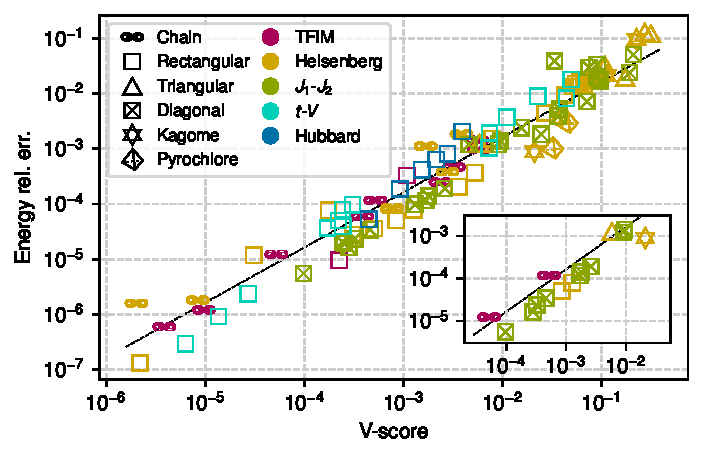
\includegraphics[width=0.8\linewidth]{ch10/v_score_rel_err.pdf}
\caption[Comparison of V-score and energy relative error]{
Comparison of V-score and energy relative error for systems whose exact solutions from ED or QMC are available.
The black dashed line is the least-squares fit.
The inset focuses on PQC results simulated on classical hardware without noise.
This figure is reproduced from Fig.~2 in Ref.~\cite{wu2023variational}.
}
\label{fig:v-score-rel-err}
\end{figure}

\begin{figure}[htb]
\centering
\hspace*{-0.05\linewidth}
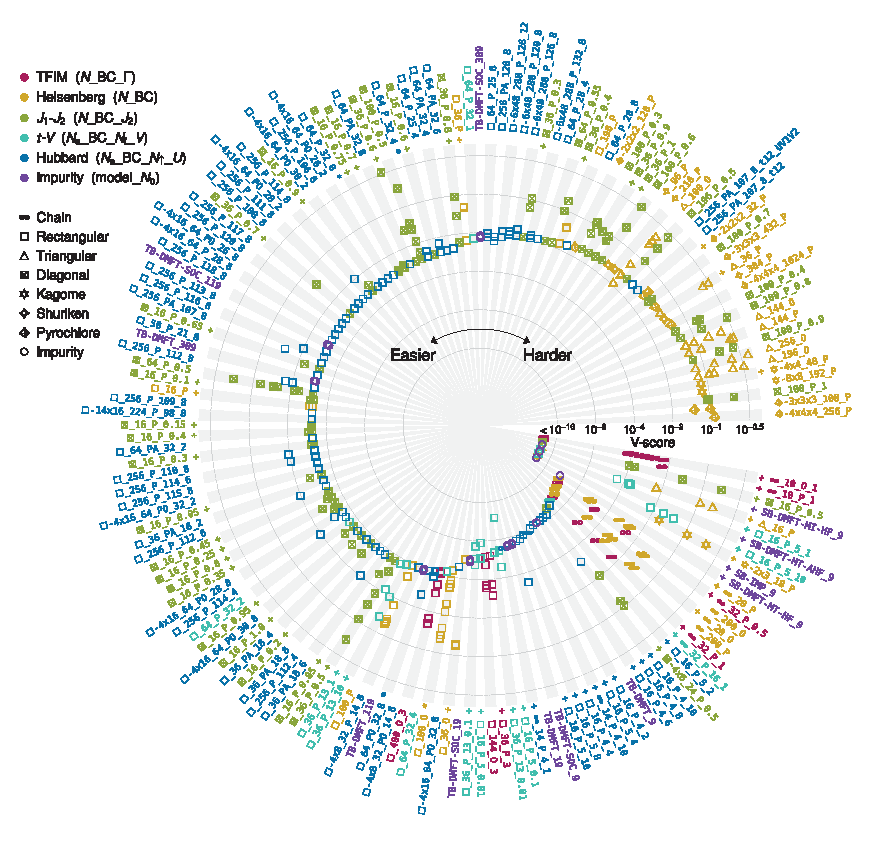
\includegraphics[width=1.05\linewidth]{ch10/v_score_polar_doubly_log.pdf}
\caption[Overview of VarBench results]{
Overview of the complete benchmark results.
Each slice in the radial direction contains different variational methods for a given Hamiltonian. The bold marker indicates the method with the lowest variational energy (rather than the lowest V-score), which defines the V-score for the Hamiltonian and determines its clockwise ranking.
The radial axis uses the doubly log scale to show the results across a wide range of V-score magnitude.
The results with V-scores less than $10^{-16}$ are indistinguishable from the exact solutions due to limited numerical precision.
The label outside each slice is the name of the Hamiltonian in the dataset, which describes the lattice geometry, the lattice size $N_\text{s}$, the boundary conditions (BC), and the Hamiltonian parameters such as the interaction strength ($\Gamma$, $J_2$, $V$, $U$) and the number of particles ($N_\mathrm{f}$, $N_{\uparrow}$, $N_\mathrm{b}$).
The BC can be O (open), P (periodic), A (anti-periodic) on each dimension.
The `\texttt{+}' marker near the label indicates that an ED solution is available for that Hamiltonian, and the `\texttt{\textasteriskcentered}' marker indicates a numerically exact QMC solution.
This figure is reproduced from Fig.~3 in Ref.~\cite{wu2023variational}.
}
\label{fig:v-score}
\end{figure}

\begin{figure}[htb]
\centering
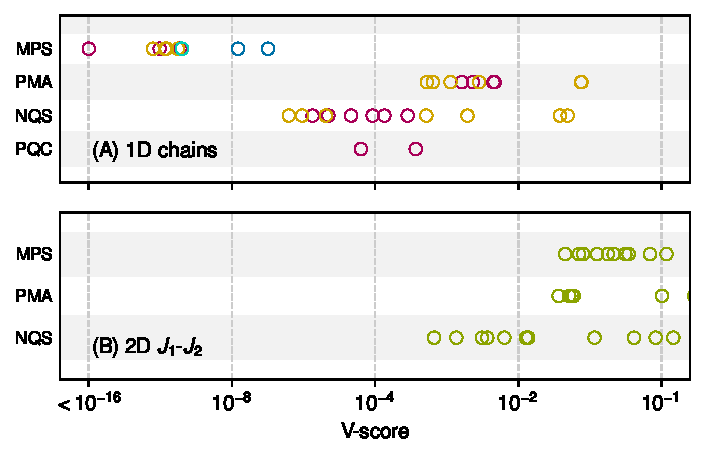
\includegraphics[width=0.8\linewidth]{ch10/v_score_method_doubly_log.pdf}
\caption[V-scores of different methods]{
V-scores classified by variational methods, including matrix product state (MPS), physically motivated ansatz (PMA), neural quantum state (NQS), and parameterized quantum circuit (PQC), on (a) 1D chains and (b) 2D $J_1$-$J_2$ models.
The $x$-axis uses the doubly log scale to show the results across a wide range of V-score magnitude.
}
\label{fig:v-score-method}
\end{figure}

\section{Difficulty of Hamiltonian}

\begin{figure}[htb]
\centering
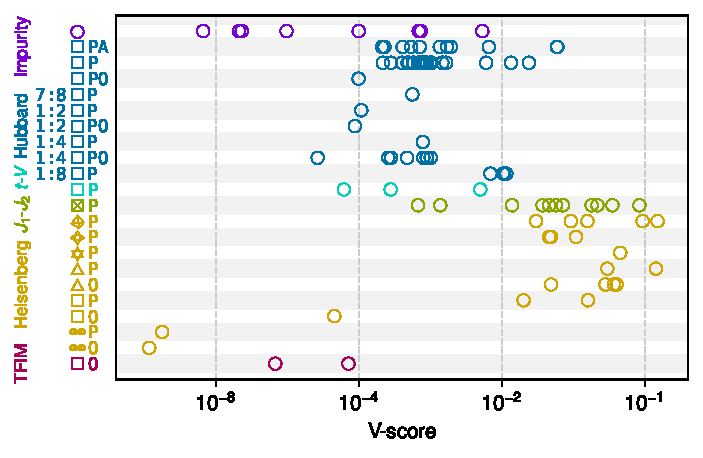
\includegraphics[width=0.8\linewidth]{ch10/v_score_ham_no_ed_doubly_log.pdf}
\caption[V-scores of different Hamiltonians]{
V-scores classified by Hamiltonian types and lattice geometries.
A Hamiltonian's V-score is defined as the V-score of the available variational method with the lowest energy on this Hamiltonian.
Only the Hamiltonians without ED results are shown.
The $x$-axis uses the doubly log scale to show the results across a wide range of V-score magnitude.
The ratios to the left of the lattice icons are aspect ratios of rectangular lattices. The letters to the right are boundary conditions, which can be O (open), P (periodic), A (anti-periodic) on each dimension.
This figure is reproduced from Fig.~4 in Ref.~\cite{wu2023variational}.
}
\label{fig:v-score-ham}
\end{figure}
